\subsection{فریم‌ورک ساخت الگوهای معماری}
\label{ZalewskiFramework}
\begin{RTL}
\lr{Zalewski} در \cite{ref2}
یک معماری برای سیستم‌های نهفته بی‌درنگ معرفی می‌کند
که آن قدر کلی بیان‌شده که از آن می‌توان به عنوان یک
فریم‌ورک برای ساخت الگوهای جدید استفاده کرد.
او ساختار خود را مبنی بر ارتباط سیستم‌های بی‌درنگ با
دنیای بیرون از خود می‌سازد. ساختار پیشنهادی او در شکل
\ref{ZalewskiFig} نمایش داده‌شده. 
\end{RTL}
\begin{figure}[h!]
\centering
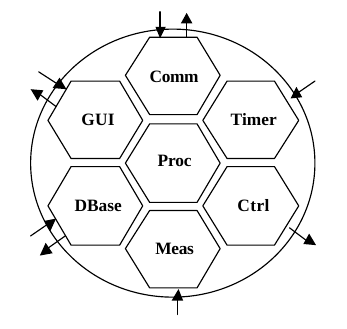
\includegraphics[]{images/zelawski-architecture.png}
\caption{معماری پیشنهادی \lr{Zalewski} \cite{ref2}}
\label{ZalewskiFig}
\end{figure}
\begin{RTL}
در این ساختار، \lr{Comm} برای ارتباط با دیگر
ساختارهای کنترلی با استفاده از یک شبکه ارتباطی،
\lr{GUI} برای ارتباط با کاربر سیستم،
\lr{DBase} برای ارتباط با دیتابیس،
\lr{Meas} برای ارتباط با سنسورها،
\lr{Ctrl} برای کنترل و \lr{Actuate}کردن
بخش‌های سیستم،
\lr{Timer} برای ارتباط با \lr{Timer} سیستم
بی‌درنگ و \lr{Proc} برای انجام پردازش‌های درونی سیستم
تعریف شده‌اند.
\end{RTL}